\documentclass{amsart}
\usepackage{graphicx}
\usepackage{caption}
\usepackage{subcaption}
\graphicspath{ {./img/} }

\usepackage{pgfplots}
\pgfplotsset{compat=1.18}
\usepackage{wrapfig}

\title{CSE306 - Assignment 2}
\author{Doan Dai Nguyen}

\begin{document}

\maketitle

In this second assignment, I have implemented the following tools and features.

\begin{itemize}
    \item Voronoi diagram solver, using Sutherland-Hodgman polygon clipping algorithm;
    \item A small header-only library for kd-tree to speed up the Voronoi diagram solver;
    \item Extension to Power diagram and weight optimisation with L-BFGS;
    \item Semi-discrete optimal transport fluid simulator with free surfaces;
\end{itemize}

The assignment was done in 734 lines of code, including 16 lines of code in \texttt{main.cpp} and 718 lines of code from 6 files in \texttt{./classes}. The project was compiled with C++20, and the following compiler flags

\texttt{-fopenmp -O3 -fcf-protection=none -march=native -mtune=native \\-fno-math-errno}

The rendering was done one a laptop with Intel Core i7-10710 CPU, 12 cores with 1.6 GHz. No GPU was used for the rendering in this report.

\begin{figure}
    \centering
    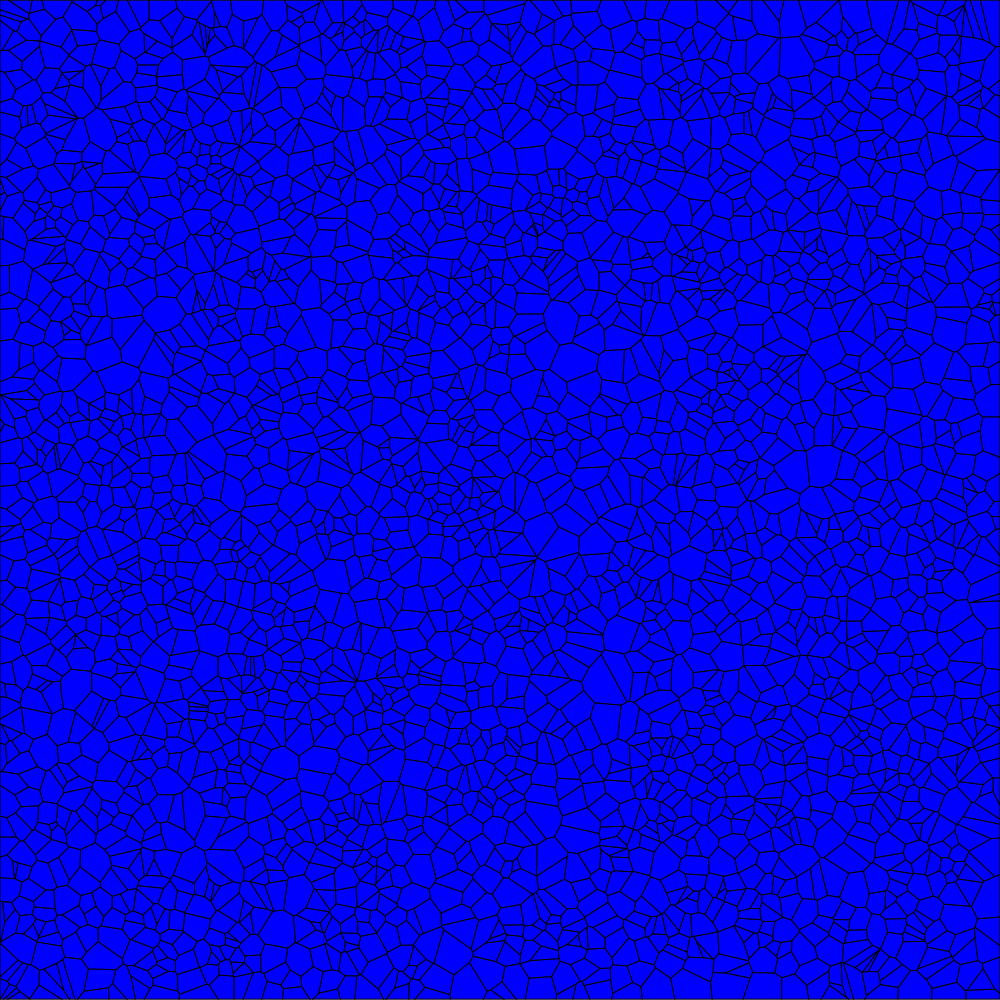
\includegraphics[width=0.72\textwidth]{img/voronoi_p.png}
    \caption{Voronoi diagram of 3000 points. Runtime was 0.058 with kd-tree, and 0.738 seconds without kd-tree.}
    \label{fig1}
\end{figure}

\begin{figure}
    \centering
    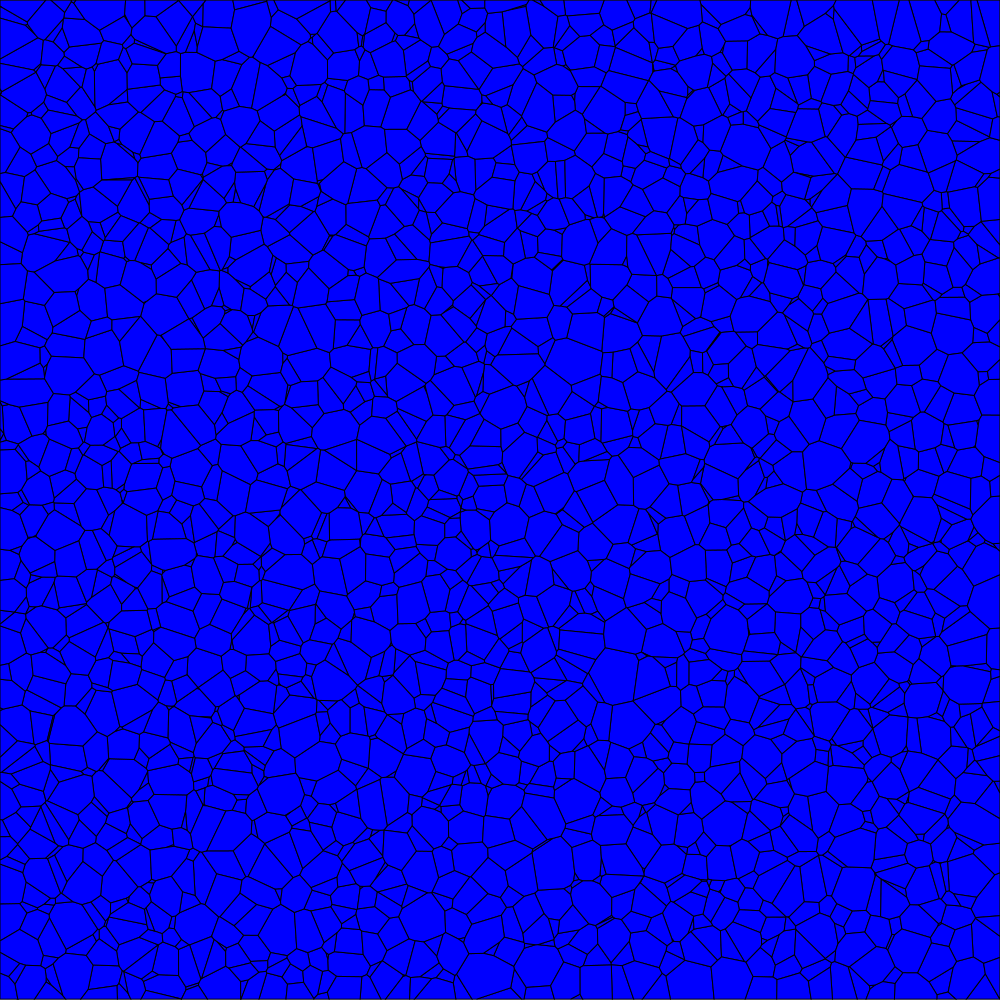
\includegraphics[width=0.65\textwidth]{img/voronoi.png}
    \caption{Power diagram of the same 3000 points as in Figure \ref{fig1} but with random weights. Runtime was 0.068 seconds with kd-tree, and 0.869 seconds without kd-tree.}
\end{figure}

\begin{figure}
    \centering
    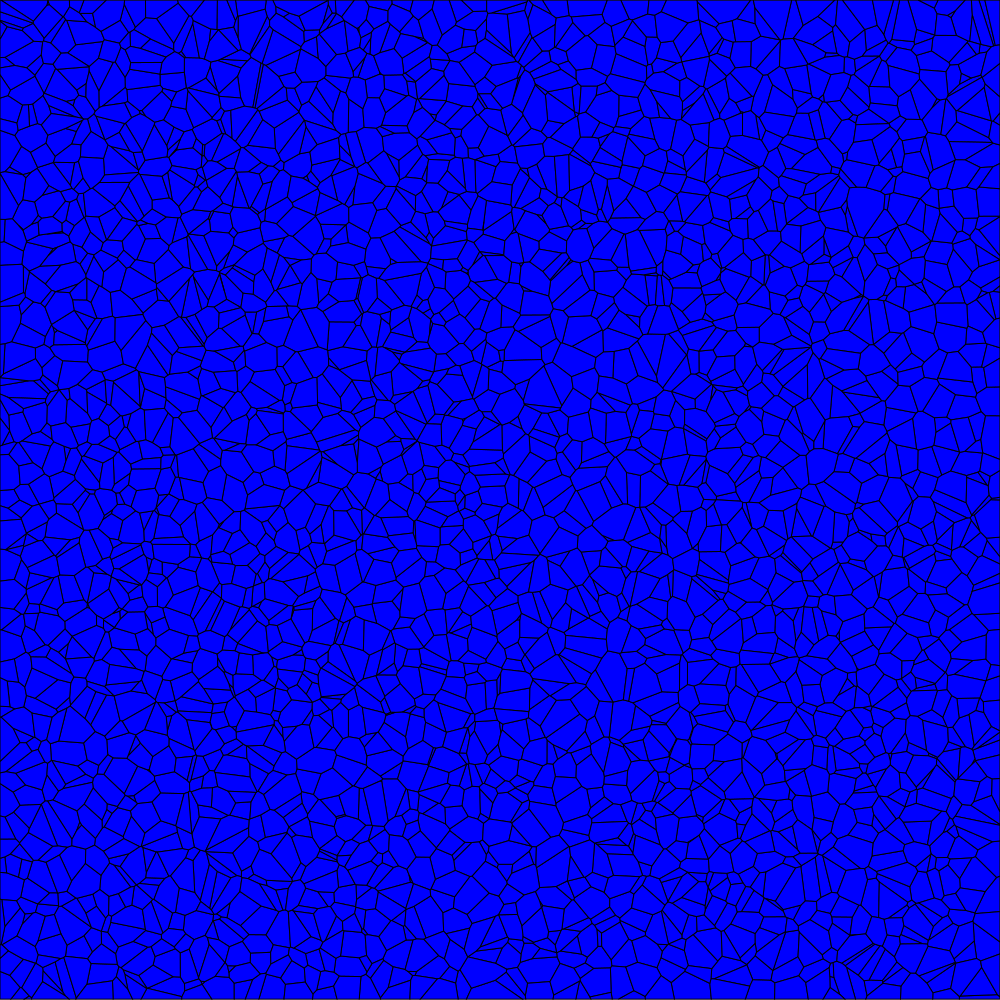
\includegraphics[width=0.65\textwidth]{img/optimal_transport.png}
    \caption{Power diagram of the same 3000 points as in Figure \ref{fig1} but with weights optimised with Optimal transport and L-BFGS. Runtime was 0.725 with kd-tree, and 42.841 seconds without kd-tree.}
\end{figure}

I also conduct some experiments to find the optimal value for $k$, the number of nearest neighbor to be requested from kd-tree. Experiments show that the distribution of number of neighbours needed for a given point is independent from the number of points in the set, thus assuming there is a fixed discrete distribution $p$, such that $p_n$ is the probability that we need $n$ neighbours.

Let $C(k)$ be the cost to request $k$ nearest neighbours from kd-tree. Carrying out complexity analysis should show that $C(k) = A + Bk\log k$ where $A$ is the cost of traversing through the kd-tree, and $Bk\log k$ is the cost of maintaining the priority queue. Then, approximating $C(mk) = mC(k)$ for integers $m$, and let $D(n)$ be the cost of finding neighbours until having at least $n$ neighbours, modulo some rounding, we have $D(mk) = C(k) + C(2k) + ... + C(mk) = \frac{m(m+1)}{2}C(k)$, or $D(n) = \frac{n(n+k)}{2k^2} C(k)$.

Then 
\begin{align*}
    \mathbb{E}(D(n)) 
    & = \sum_n p_n D(n) = \sum_n p_n \frac{n(n+k)}{2k^2} C(k) \\
    & = C(k) \left(\sum_n p_n \frac{n(n+k)}{2k^2}\right) = \frac{C(k)}{2} \left(\frac{1}{k^2} \sum_n p_n n^2 + \frac{1}{k} \sum_n p_n n \right) \\
    & = \frac{A + Bk\log k}{2} \left(\frac{1}{k^2} C + \frac{1}{k} D \right),
\end{align*}
where $A, B, C, D$ are all constants and independent of $k$. This final formula suggests that there should be a fixed optimal value for $k$. Some more experiments show that $k = 15$ gives better performances than other values tested.

\begin{figure}
    \centering
    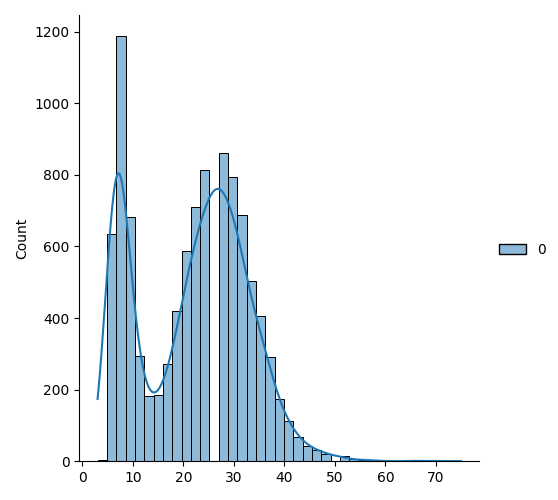
\includegraphics[width=.75\textwidth]{img/plot.png}
    \caption{Number of neighbours needed to be requested from kd-tree for a typical set of 300 points.}
\end{figure}

\end{document}
